%%%%%%%%%%%%%%%%%%%%%%%%%%%%%%%%%%%%%%%%%%%%%%%%%%%%%%%%%%%%%%%%%%%%%%%%%%%%%%%%
\chapter*{Основная часть} % Заголовок
\addcontentsline{toc}{chapter}{Основная часть} % Добавить в оглавление
\refstepcounter{chapter} % Счётчик

%%%%%%%%%%%%%%%%%%%%%%%%%%%%%%%%%%%%%%%%%%%%%%%%%%%%%%%%%%%%%%%%%%%%%%%%%%%%%%%%
%%%%%%%%%%%%%%%%%%%%%%%%%%%%%%%%%%%%%%%%%%%%%%%%%%%%%%%%%%%%%%%%%%%%%%%%%%%%%%%%
\section{Метод полностью параллельной разностной эволюции} \label{s1}

Метод ППРЭ успешно применялся в~различных задачах~\cite{bib3,bib4}.
Совершенствование методов минимизации для нахождения параметров генных 
регуляторных сетей требует наличия набора тестов для оценки новых алгоритмов 
и~реализаций и~сравнения с~предшествующими. 

В самом общем смысле класс рассматриваемых задач можно назвать задачами 
поиска глобального минимума некоторого функционала качества (или функции). 
Способов решения таких задач достаточно много. В работе рассматривается 
модификация стохастического итерационного метода разностной эволюции (РЭ). 
Идея метода РЭ, предложенного Р.~Сторном~\cite{bib1}, заключается в 
моделировании популяции индивидуумов (а точнее, векторов их определяющих). 
Популяция меняется от поколения к поколению, при этом индивидуумы скрещиваются 
и мутируют. 

Метод РЭ имеет набор управляющих параметров (например, размер популяции 
или количество старейших индивидуумов, заменяемых на новые), от которых сильно 
зависит скорость работы и сходимость. В~\cite{bibZaharie} была предложена 
адаптивная схема выбора управляющих параметров метода РЭ. В работе~\cite{bibTM}
введено тригонометрическое преобразование (мутация) вектора-индивидуума 
зависящее от функционала качества. 

В данной работе рассматривается метод ППРЭ~\cite{bib2,bib5}. 
Возраст индивидуума — количество итераций, которые он существует. 
Спустя определённое количество итераций $es\_lambda$ самых старых
индивидуумов заменяется на $es\_lambda$ самых «лучших».

\clearpage
%%%%%%%%%%%%%%%%%%%%%%%%%%%%%%%%%%%%%%%%%%%%%%%%%%%%%%%%%%%%%%%%%%%%%%%%%%%%%%%%
%%%%%%%%%%%%%%%%%%%%%%%%%%%%%%%%%%%%%%%%%%%%%%%%%%%%%%%%%%%%%%%%%%%%%%%%%%%%%%%%
\section{Экспериментальные данные (DREAM)} \label{s2}

Проект DREAM (Dialogue for Reverse Engineering Assessment and Methods)
предоставляет унифицированные экспериментальные данные для тестирования 
алгоритмов. Каждое «испытание» — некая формализованная задача,
которую предлагается решить независимым группам исследователей. Лучшие 
решения в результате публикуются \cite{bib6}. 

В рамках этой работы требуется подобрать близкие к оптимальным значения 
параметров ППРЭ, используя в качестве тестовых задач результаты DREAM6.

%%%%%%%%%%%%%%%%%%%%%%%%%%%%%%%%%%%%%%%%%%%%%%%%%%%%%%%%%%%%%%%%%%%%%%%%%%%%%%%%
\subsection{Постановка задачи} \label{s2_1}

Эта задача принадлежит области обратной инженерии генно-регуляторных сетей. 
Предполагается, что топология генной сети уже определена с достаточным уровнем 
правдоподобия, и теперь требуется охарактеризовать параметры (кинетику) 
этой сети.

Здесь есть два ключевых аспекта, которые требуют внимания: задача оценки 
параметров модели по данной структуре модели, а так же задача проектирования 
наиболее информативных экспериментов для получения неизвестных параметров. 

Итак, даны структуры трёх генно-регуляторных сетей, от участников требуется 
разработать и/или применять методы оптимизации, чтобы точно оценить 
параметры моделей а так же прогнозировать результаты возмущений в этих моделях.

Эти две задачи и являются областью исследования DREAM6. Однако, для тестирования
ППРЭ потребуется рассмотреть лишь первую задачу.

%%%%%%%%%%%%%%%%%%%%%%%%%%%%%%%%%%%%%%%%%%%%%%%%%%%%%%%%%%%%%%%%%%%%%%%%%%%%%%%%
\subsection{Модели генных сетей: Представление данных} \label{s2_2}

Полные структуры генных сетей представлены в формате sbml, tic, и в графическом 
формате. Пример такого представления для первой генной сети приведён на 
рисунке~\ref{img:GrnImage}.

\begin{figure}[h]
  \center{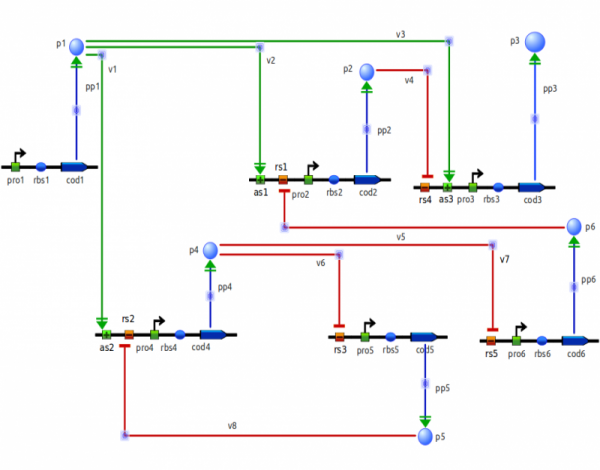
\includegraphics[width=14cm]{model1-600x470.png}}
  \caption{Пример графического представления для первой генной сети}
  \label{img:GrnImage}
\end{figure}

\begin{figure}[h]
  \begin{minipage}[h]{0.34\linewidth}
    \center{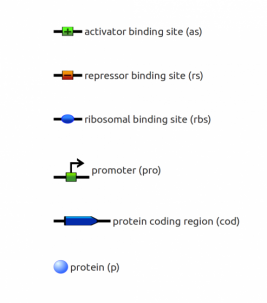
\includegraphics[height=8cm]{diagram_key-267x303.png}}
    \caption{Аннотация к графическому представлению}
    \label{img:GrnImageDesc}
  \end{minipage}
  \hfill
  \begin{minipage}[h]{0.64\linewidth}
    \center{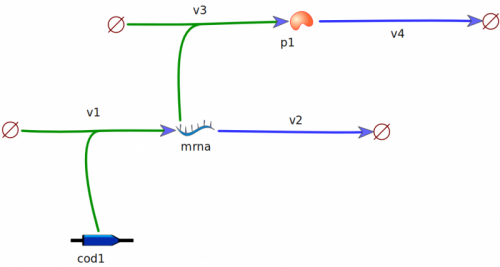
\includegraphics[height=6cm]{protein_production_subfigure-500x267.png}}
    \caption{Транскрипция и трансляция, не показанные на схеме генной сети}
    \label{img:GrnImageTT}
  \end{minipage}
\end{figure}

Для каждой сети предоставляется файл (.m) с описанием модели в 
синтаксисе MATLAB. Все переменные помечены в соответствии с их типом. 
Например, переменные, означающие концентрацию белка, помечены как 
$p1$,~$p2$,~...~$p6$. 

Значения каждого символа в генной сети подробно 
объясняются в легенде (рис.~\ref{img:GrnImageDesc}). В скобках перечислены 
префиксы к переменным модели. Линии, соединяющие кодирующую белок 
последовательность с белком, обозначены префиксом «pp». Генерация белка состоит 
из двух логических частей: транскрипция и трансляция. Для простоты, эти два 
этапа, изображённые на схеме~\ref{img:GrnImageTT}, не показаны в диаграмме 
генной сети. 

Имена переменных для мРНК, для результата транскрипции кодирующей 
последовательности, так же имеют соответствующий префикс «pp». Например, мРНК, 
соответствующая $pp3$ будет именована как $pp3\_mrna$.

%%%%%%%%%%%%%%%%%%%%%%%%%%%%%%%%%%%%%%%%%%%%%%%%%%%%%%%%%%%%%%%%%%%%%%%%%%%%%%%%
\subsection{Параметры генных сетей} \label{s2_3}

Генная сеть характеризуется топологией (структурой), о которой говорилось выше, 
и набором параметров — скорость трансляции, транскрипции, и параметров, 
отвечающих за сайты связывания рибосом. Если все эти параметры и начальные 
данные (начальные концентрации мРНК) определены, рассматривается поведение 
генной сети на фиксированном интервале времени. Под поведением здесь имеется 
ввиду динамика изменения концентраций мРНК и белка каждого типа.

Таким образом, каждая генная сеть с заданными параметрами порождает матрицу, 
содержащую набор концентраций для фиксированных моментов времени. В DREAM6 от
участников требуется решить обратную задачу: по данной матрице концентраций 
(пример матрицы~\ref{mRNAtable}) предоставить набор параметров сети.

%%%%%%%%%%%%%%%%%%%%%%%%%%%%%%%%%%%%%%%%%%%%%%%%%%%%%%%%%%%%%%%%%%%%%%%%%%%%%%%%
\subsection{Начальные данные и возмущения} \label{s2_4}

Наборы данных, которые предоставляются в качестве входных для оценки параметров 
были сформированы искусственно, путем моделирования, с учётом различных 
возмущений (зашумлений) в генной сети — делеции гена, мРНК нокдаун и изменение 
активности сайтов связывания рибосом. 

Оговорено, что во всех случаях возмущения могут затрагивать только один ген. 
Удаление гена приводит к полной ликвидации как мРНК, так и белка целевого гена. 
В случае миРНК, мРНК деградирует (фиксированное уменьшение в 5 раз), что 
приводит к уменьшению как мРНК так и концентрации соответствующего белка.

\begin{table}[h]
  \centering
    \begin{tabular}{l|llllll}
        0.0	  & 0.0    & 0.0   & 0.041  & 0.16  & 0.189  & 0.048 \\
        2.0	  & 2.754  & 4.01  & 4.531  & 0.30  & 0.221  & 0.006 \\
        4.0	  & 2.958  & 2.96  & 0.911  & 0.06  & 0.522  & 0.39  \\
        6.0	  & 4.058  & 2.18  & 0.457  & 0.07  & 1.609  & 1.266 \\
        8.0	  & 3.41   & 1.06  & 0.649  & 0.08  & 2.627  & 2.253 \\
        10.0  & 3.459  & 0.68  & 4.398  & 0.07  & 2.979  & 3.811 \\
        12.0  & 2.453  & 0.67  & 6.734  & 0.27  & 2.618  & 2.983 \\
        14.0  & 1.234  & 0.43  & 5.971  & 0.02  & 2.443  & 3.025 \\
        16.0  & 2.385  & 0.43  & 4.606  & 0.0   & 1.821  & 2.823 \\
        18.0  & 3.691  & 0.52  & 5.827  & 0.0   & 3.444  & 2.386 \\
        20.0  & 3.252  & 0.4   & 8.947  & 0.0   & 4.358  & 3.666 
    \end{tabular}
  \caption{Пример таблицы концентраций мРНК для первой генной сети}
  \label{mRNAtable}
\end{table}

\clearpage
%%%%%%%%%%%%%%%%%%%%%%%%%%%%%%%%%%%%%%%%%%%%%%%%%%%%%%%%%%%%%%%%%%%%%%%%%%%%%%%%
%%%%%%%%%%%%%%%%%%%%%%%%%%%%%%%%%%%%%%%%%%%%%%%%%%%%%%%%%%%%%%%%%%%%%%%%%%%%%%%%
\section{Численные эксперименты} \label{s3}

%%%%%%%%%%%%%%%%%%%%%%%%%%%%%%%%%%%%%%%%%%%%%%%%%%%%%%%%%%%%%%%%%%%%%%%%%%%%%%%%
\subsection{Постановка задачи в терминах метода ППРЭ} \label{s3_1}

Метод ППРЭ ищет минимум функционала качества по списку параметров. Параметры — 
неопределённые параметры генной сети, о которых говорилось в предыдущей главе. 

За функционал качества выбирается расстояние между заранее определённой матрицей 
концентраций $W$ (см.~\ref{s2_3}) и матрицей концентраций, полученной с текущими 
параметрами. При этом расстояние понимается как сумма квадратов поэлементных 
разностей двух матриц. 

Как уже было сказано, в качестве оценки работы ППРЭ используются две 
характеристики: 
\begin{enumerate}
	\item Расстояние между известной и полученной матрицами концентраций. Т.е. 
	функционал качества.
	\item Расстояние между известными и полученными параметрами
\end{enumerate}

Более формально: генная сеть, при выборе вектора параметров $p$ и задании
вектора начальных условий $e$ пораждает дифференциальное уравнение $ODE(p,e)$. В 
силу однозначности начальных данных, решение этого уравнения единственно. 
Решение — динамика изменений концентраций мРНК и соответствующих им белоков. При
фиксированном интервале времени и разбиении решение есть матрица концентраций 
$M^{(p,e)}$.

\[ (p,e) \rightarrow ODE(p,e) \rightarrow M^{(p,e)} \]

Так как вектор начальных условий $e$ неизменен и определён, конструкция 
упрощается:

\[ p \rightarrow ODE(p) \rightarrow M^p \]

Функционал качества для метода ППРЭ есть расстояние:

\[ \sum\limits_{i,j}(M_{i,j}^p - W_{i,j})^2 \]

Теперь обозначим расстояние между известными $p^*$ и текущими параметрами $p$ 
как $\rho(p,p^*)$, тогда каждый вектор параметров $p$ пораждает два числа (две 
характеристики, о которых говорилось выше):

\[ 
p \rightarrow ODE(p) \rightarrow M^p 
\rightarrow \{ \sum\limits_{i,j}(M_{i,j}^p - W_{i,j})^2 , \rho(p,p^*) \}
\]

%%%%%%%%%%%%%%%%%%%%%%%%%%%%%%%%%%%%%%%%%%%%%%%%%%%%%%%%%%%%%%%%%%%%%%%%%%%%%%%%
\subsection{Прогонка управляющих параметров ППРЭ} \label{s3_2}

В качестве критерия остановки было выбрано время, прошедшее с момента начала 
работы. 

Для всех трёх моделей было зафиксировано $population\_size = 150$ 
и~варьировалось $es\_lambda = 2,15,45$. Всего было проведено 20 запусков для 
каждой модели. Результаты сходимости представлены в приложниее 
на рисунках~(\ref{img:pm1},~\ref{img:pm2},~\ref{img:pm3}).

В левом столбце представлена зависимость значения минимизируемого функционала 
(вертикаль) от времени (горизонталь). В правом — расстояние $\rho$ между 
известными параметрами генной сети и параметрами, найденными методом ППРЭ.

Далее (рис.~\ref{img:em1},~\ref{img:em2},~\ref{img:em3}) представлены результаты
работы алогритма при изменении параметра $population\_size$. Аннотация 
аналогична.

Сходимость значий функционала очевидна.

\clearpage
%%%%%%%%%%%%%%%%%%%%%%%%%%%%%%%%%%%%%%%%%%%%%%%%%%%%%%%%%%%%%%%%%%%%%%%%%%%%%%%%
